\documentclass[12pt]{article}
\usepackage{float}
\usepackage{caption}
\usepackage{times}
\usepackage{natbib}
\usepackage{graphicx}
\usepackage[section]{placeins}
\usepackage{indentfirst}
\usepackage{fancyhdr}
\usepackage{xcolor}
\usepackage{enumitem}
\usepackage{listings}
\usepackage{color}
\usepackage[hyphens,spaces,obeyspaces]{url}
\usepackage{hyperref}
\pagenumbering{roman}
\hypersetup{
    colorlinks=true,
    linkcolor=blue,
    urlcolor=blue,
    citecolor = gray,
    linktoc=all
}
\lstset { %
	language=C++,
	backgroundcolor=\color{black!5}, % set backgroundcolor
	basicstyle=\footnotesize,% basic font setting
}
\pagestyle{fancy}
\fancyhf{}
\rhead{\textit{\color{gray}\today}}
\lhead{\textit{\color{gray}C++14 Software Transactional Memory}}
\rfoot{Page \thepage}
\lfoot{\color{gray}\LaTeX}

\pagenumbering{roman}
\begin{document}

\begin{titlepage}
	\begin{center}
	\line(1,0){350}\\
	[0.3 cm]
	\huge{\textbf{Software Transactional Memory\\[0.3 cm]C++14 STM\\ }} 
	\line(1,0){200}\\
	[0.3 cm]
	\huge{\textbf{Functional Specification }} 
		\begin{LARGE}
		\\[0.3 cm]Zoltan Fuzesi\\
		\today
		\end{LARGE}
		
		\begin{LARGE}
		\line(1,0){150}\\
		[1.0 cm]
		Student ID: C00197361\\
		Supervisor: Joseph Kehoe\\
		\color{gray}Institute of Technology Carlow\\
		\color{gray}Software Engineering
		\end{LARGE}
		
\begin{figure}[h!]
\centering

\includegraphics[scale=0.7]{Pictures/carlow.png}

\end{figure}
		
	\end{center}
\end{titlepage}

\tableofcontents


\clearpage
\pagenumbering{arabic}
\setcounter{page}{1}
\section{Introduction}
Since the modern computers has more the one core embedded into the CPU, the concurrent and parallel programming is the way to keep the CPU throughput as high as possible and create faster applications. The concurrent and parallel programming requires to sharing memory spaces between processes, cores associated with a running application.\\

The purpose of this project to implement a Software Transactional Memory library in C++14 programming language, to enable other programs to include and use this library as a lock free solution, to use for concurrent programming to protect shared memory spaces, which are used by an application. Because the STM library implementation does not require graphical user interface, database connection and network connectivities, the implementation is limited only for logical C++ code solution, that can be used and tested by an external application. The library itself will be a file with '*.a' or '*.so' extension on Linux , that need to be placed into the file system in the Linux operating (shared *so file) system or placed to the C++ project folder structure (static *.a) to link together with the application. So, as the part of the project, it is require to create a test application to illustrate and test the library usage.\\

As the mandatory requirements, the project will be fully documented by the Doxygen document generator tool, to provide the description of the available interface functions to other programmers, if they intend to use the library. Create a test application to demonstrate the library usage.\\

To make it available on different operating systems, the library will be developed and tested on Linux, Windows and MAC OSX to make it available in cross platform versions. As a final result, create benchmarking test, to compare with other Software Transactional Memory solutions or similar systems.

\clearpage
\section{What the product can do}
The STM library will be developed in C++14 language syntax to provide lock free solution to client applications to protect shared memory within a transactional process. It will support an API interface to the applications to enable library call(s) after a transaction object has created. It will allows the transaction object to pass objects to the library, to store and make changes on them. As the part of the transaction process, the library will create a transaction, make shared local data structure to store objects involved in the transactions, and when finish with the changes, try to end the transaction and only write changes in the memory spaces if the transaction not fail. When the transaction fails, then need to restart the process. Because the STM library provide transactional environment to the client applications, the programmers don't need to worry about to use mutex, semaphore and can avoid of deadlock and livelock situations.

\section{Functional description}
Software Transactional Memory allows to compose several actions, that all can be execute together and run as a single transaction. The library will provide public API functions, such as register, load, store and commit to use values/pointers to work with, and these functions will working together to achieve the transactional behaviour. When the transaction library receive the data to work with, then will create and start a transaction. At the last step in the transaction try to commit the changes, that need to carry out on the shared data. It is involves in few inner steps such as compare the version numbers and update the changes. If the version number are different between the working object and the global object, then the transaction will restart. The transaction steps are detailed in below.

\begin{figure}[h!]
\centering
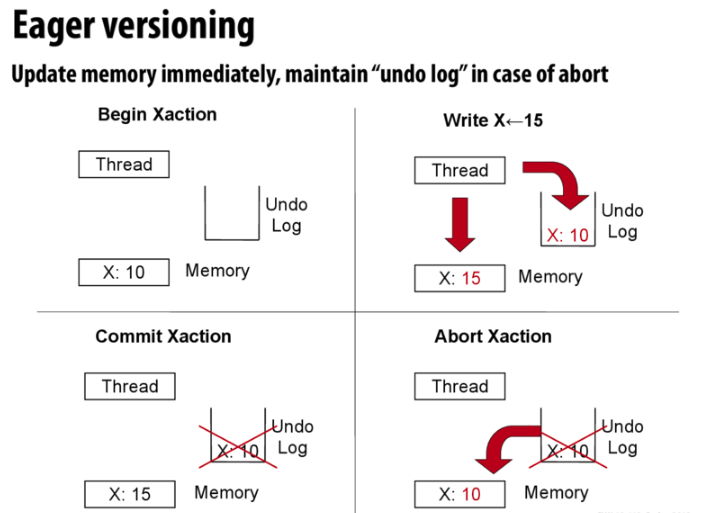
\includegraphics[scale=0.4]{Pictures/eager.png}
\caption{\textit{\color{gray}A simple example of eager version. \cite{Xelblade}.}}
\end{figure}

\begin{figure}[h!]
\centering
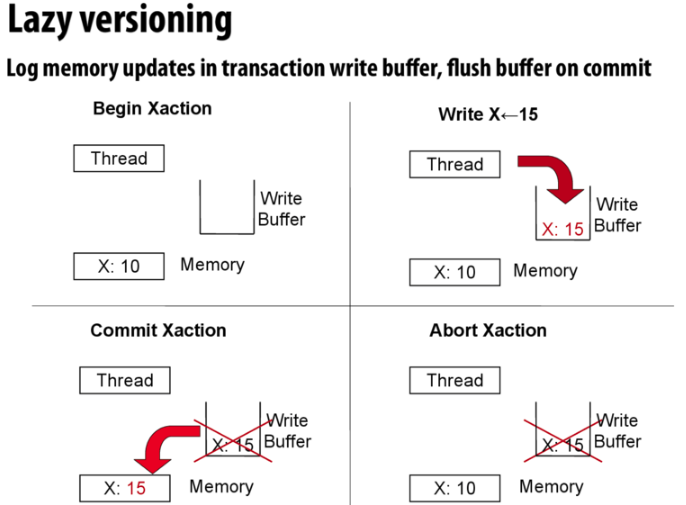
\includegraphics[scale=0.4]{Pictures/lazy.png}
\caption{\textit{\color{gray}A simple example of lazy version. \cite{Xelblade}.}}
\end{figure}

\clearpage
\subsection{Create transaction}
When the external program creates an object of the transaction library, it's functions available to the transaction object. The transaction object able to pass the required values to the transaction library, to make changes on them. When the object calls the function and passing the values/object to the transactional memory library, the transaction has created and the transaction life cycle begin.\textit{\color{gray}Figure 3}

\begin{figure}[h!]
\centering
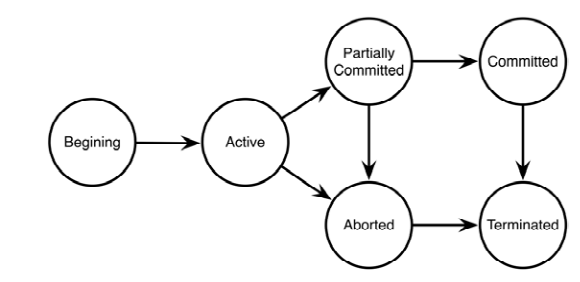
\includegraphics[scale=0.4]{Pictures/begin.png}
\caption{\textit{\color{gray}Transaction basic life cycle. \cite{DLUATM}.}}
\end{figure}

The values/object received by the transactional memory library, it creates a copy of the value/object to the local shared data set to work with. It is an important step, since the library not making changes on the original value until the end of the transaction life cycle.\textit{\color{gray}Figure 4}

\begin{figure}[h!]
\centering
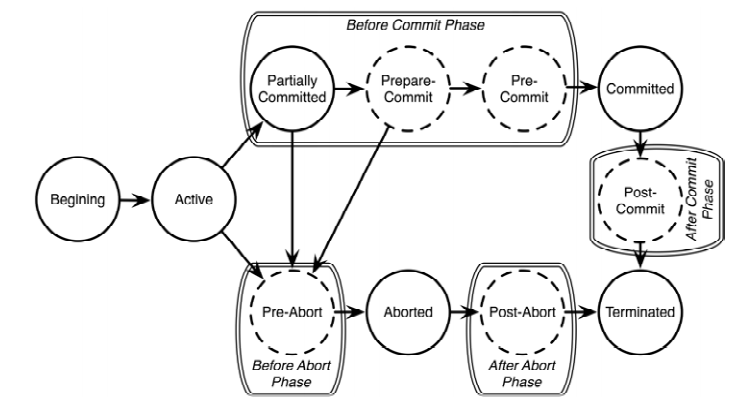
\includegraphics[scale=0.4]{Pictures/transactionLifeCycle.png}
\caption{\textit{\color{gray}Transaction life cycle states. \cite{DLUATM}.}}
\end{figure}

A copy created and associating a version number with it. This version number will be used to determine the changes on the value/object by the other transactions within the context.

\subsection{Start transaction}
When the transaction start, the library check the version number associated with the data/object, to compare against the transaction own copy. If the version numbers are not the same, then the transaction aborting and restart with the new copy of the origanl object. If the version numbers are same, then the transaction locks the global data set copy of the value/object and make the changes. Before the transaction commit, make permanent changes on the value/object used in the transaction it needs to compare the version number again to determine the conflicts.   

\subsection{Commit transaction}
This phase of the transaction, the library locks the used shared memory spaces in an atomic block, and hide from the other processes to write changes into the local data set. After the changes has made on the local data set, before finalize the write process to the destination shared memory spaces, must to determine if any other process had accessed the same data set, and made changes on it. It is happening with compare the transaction object version number with the shared memory space version number. The transaction commits the changes if no conflict detected between version numbers. When the changes has made on the shared memory space, then release the lock on the data/object and the transaction has finished.\\ 

\subsubsection{Version checking}
The version number representing the changes associated with the object accessed by the transactions. The transaction can detect the conflict early when first time accessing the value or when the transaction attempts to commit. When a transaction commit the changes, write the new values to the shared memory space, and the same time increasing the global version number to indicate to the other transactions, that some changes happened with the object. At commit time the transaction compare the local object version numbers against the global object version number. The version number in the actual transaction and the global version number associated with the object must match. If the values are not the same the transaction will be cancelled and rolling back the changes  and restart the transaction.

\begin{figure}[h!]
\centering
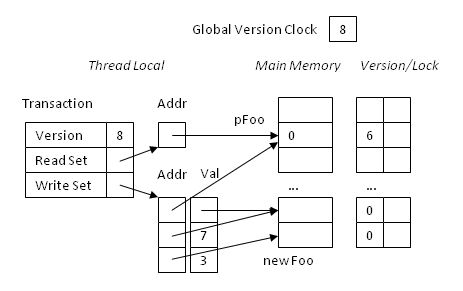
\includegraphics[scale=0.4]{Pictures/version.png}
\caption{\textit{\color{gray}Check version number. \cite{Bartosz}.}}
\end{figure}


\subsubsection{Roll-back transaction}
The roll-back part of the transaction, simply goes back to the begging of the transaction and restart the process. The library should implement some sort of checking logic, that the roll-back process must be cancelled at some stage, otherwise it can create an infinite or very long looping time in the client application.

\subsubsection{Updating}
At commit time, if the compared versions are holding same values, then the transaction updating the shared memory space on the target data set and closing the transaction. \\

The following code snippet is an atomic transaction with compiler support to change nodes in linked list structure:
\begin{lstlisting}
atomic {
  int x = node.head;
  tail = node.tail;
}
\end{lstlisting}

\section{Target users}
The potential target users can be any programmer, how planning to use concurrent programming features in their application, but in the same time they wants to avoid of the lock based programming disadvantages. Since, STM provide interface to access the built in transactional functionalities through object accessible method call, it is easy to use because only need to include the library into the client application.\\

{\setlength{\parindent}{0cm}
The potential target users can be who:
\begin{enumerate}
\item Individual programmers, software companies. 
\item Want to use transactional environment.
\item Want to avoid of lock based programming.
\item Want to use concurrent programming features in safe environment.
\item Want to avoid deadlock and livelock.
\end{enumerate}
}

\clearpage
\section{Metrics}
The C++14 Software transactional Memory project is successful, when the library working as it is expected in all circumstances. To fulfil these achievement the project must produce the following requirements:\\


\textbf{Mandatory requirements:} 
\begin{enumerate}
\item The project have to:
	\begin{itemize}
	\item Implemented Software Transactional Memory library in C++ language working on Linux platform.
	\item Documentation of the library using Doxygen documentation tool.
	\item Tutorial showing how to use the library, including test application that use the STM library.
	\end{itemize}


\textbf{Discretionary requirements:} 

\item The project have to:
	\begin{itemize}
	\item Portable : tested across multiple platform (Windows, Linux, OSX).
	\item Web site: library backed up and demonstrating it usage.
	\end{itemize}

\clearpage
\textbf{Exceptional requirements:} 

\item The project have to:
	\begin{itemize}
	\item Benchmarked : The project including benchmarking test to show the performance in different circumstances.
	\item Comparisons : Compare between other STM solutions and other approaches with usability, performance.
	\end{itemize}
\end{enumerate}

\subsubsection{FURPS}
As part of the metrics, the library should implement not functional requirements (FURPS)\cite{PPTX}
\begin{enumerate}
\item \textbf{Functionality} - The product features that represent the domain of the product solution being developed. 
\item \textbf{Usability} - Capturing and stating the requirements based on functional interface of the product and how easy to use based on the product documentation. 
\item \textbf{Reliability} -  Includes the availability, frequency of failures and recoverability if the product has unexpected failure.
\item \textbf{Performance} - Includes throughput, response time with diverse circumstances - example 10, 100 or 1000 threads are using the library with benchmarking test.
\item \textbf{Supportability} - Includes all other requirements such as 
testability, adaptability, maintainability, scalability and portability between platforms. 
\end{enumerate}

\newpage
\section{Other STM libraries}
The Software Transactional Memory was implemented in C/C++ language many time before. However, this project must produce a fully implemented STM library to support lock free transactions, possibly the library functionalities will be a bit restricted compare with the other C/C++ library implementations available. Why? Because those libraries are available years ago and developed over the time.\\

The Software Transactional Memory was implemented in many different languages as well, including C, C++, Clojure, Common Lisp, Haskell, Java, Python, Pearl and many more.

\textbf{Some C/C++ STM implementation:} 
\begin{enumerate}
\item TinySTM is a lightweight and efficient word-based STM implementation in C++.
\item libCMT based on Composed Memory Transaction written in C.
\item Intel STM Complier prototype Edition implements STM for C/C++ directly in a complier
\item stmmap based on shared memory accessing written in C.
\item TL2 transaction locking implementation of STM that’s been most widely accepted
\item CTL based on TL2 and added many extensions and optimization
\item many more
\end{enumerate}

\textbf{This project will be based on TL2 logics, which are the followings:}
\begin{enumerate}
\item Sample global version-clock.
\item Run through a speculative execution.
\item Lock the write-set.
\item Increment global version-clock.
\item Validate the read-set.
\item Commit and release the locks.
\end{enumerate}

\section{Project Iterations / Updated}
\begin{center}
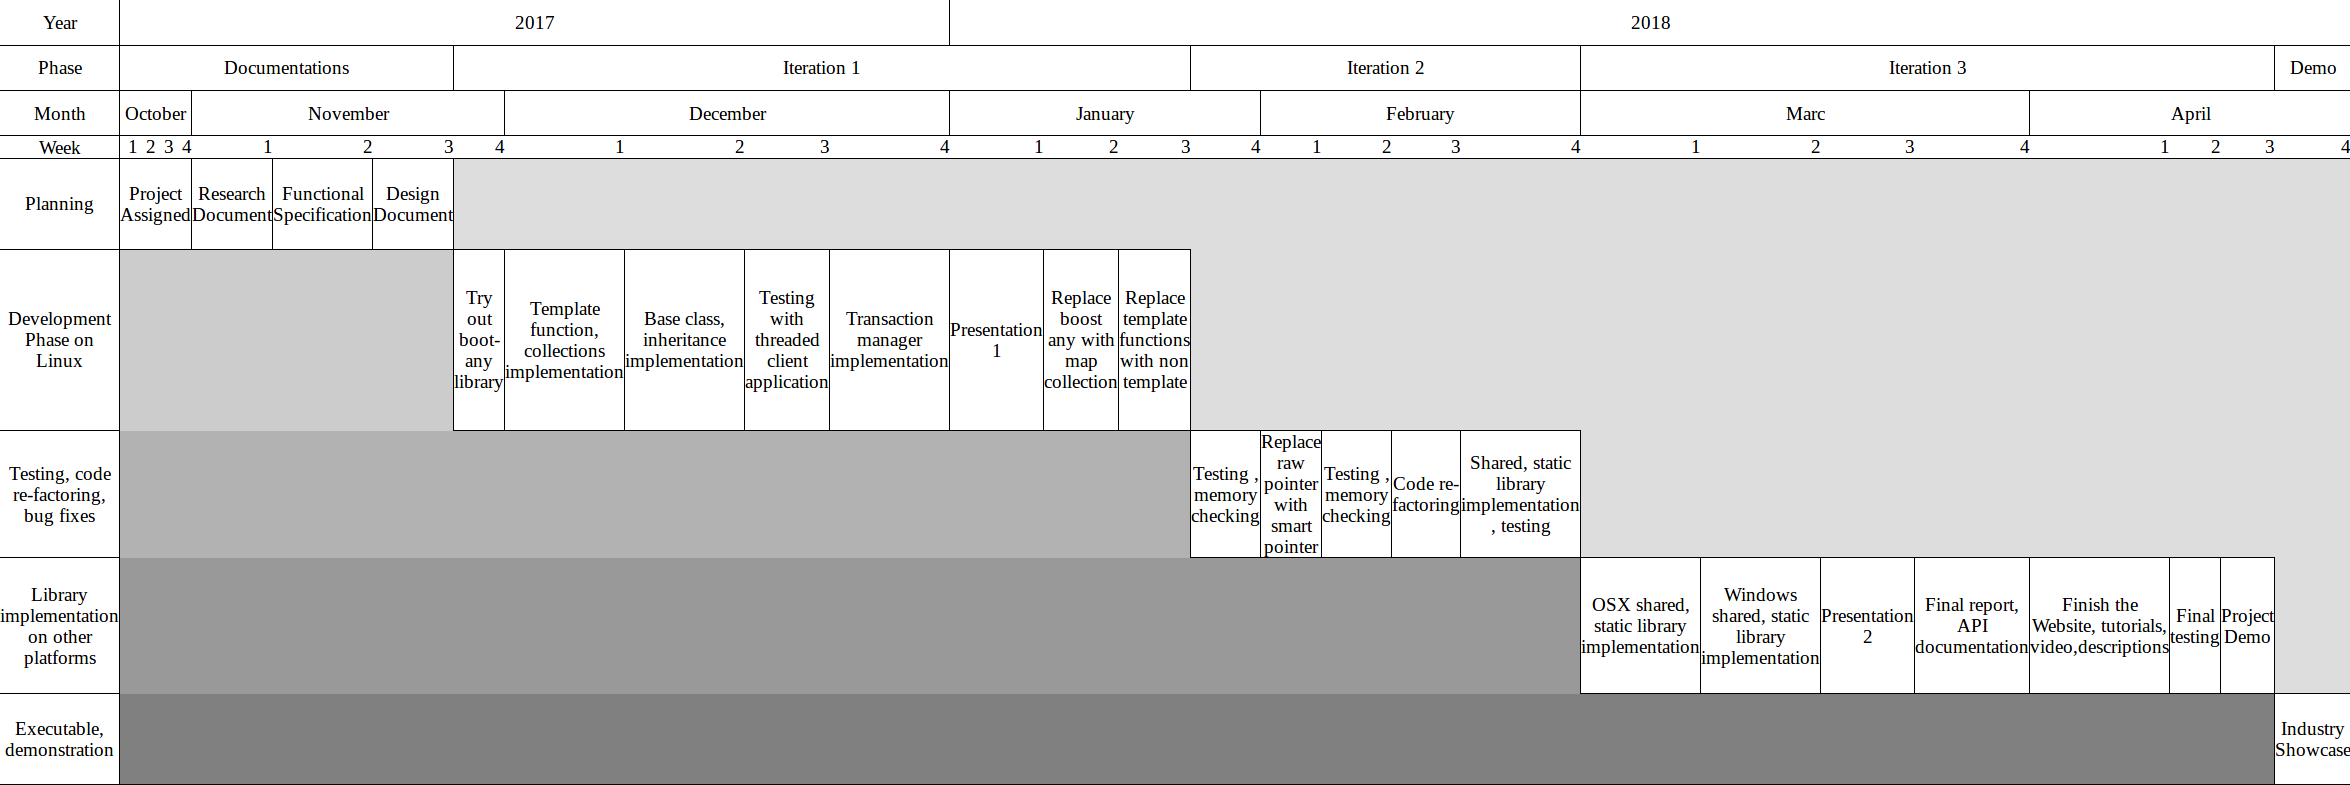
\includegraphics[angle=90,width=\textwidth,height=\textheight, height=18cm, keepaspectratio]{Pictures/gant_chart.png}
\end{center}
\newpage
\subsection{Detailed Iterations description / Updated}

\textbf{2017/2018 }
\begin{enumerate}[label*=\arabic*.]
\item October
\begin{enumerate}[label*=\arabic*.]
	\item Project assigned.
\end{enumerate}
\item November
\begin{enumerate}[label*=\arabic*.]
	\item Writing Research Document .
	\item Writing Functional Specification.
	\item Writing Design Document.
	\item \textbf{Begin Iteration 1 :} Research to find a C++ collection type to store any type of object. Try out boost-any C++ library.
\end{enumerate}
\item December 
\begin{enumerate}[label*=\arabic*.]
	\item Implementing template some functions and collections in the transaction class to store objects within the library. 
	\item Implementing the OSTM base class (blueprint of the class) virtual methods and the required unique identifier generation processes to provide unique identifier to inherited objects the intend to use with the library.
	\item First time testing the base functions with a client application, using the library files only.
	\item Implementation of the Transaction Manager to control the transactions.
\end{enumerate}
\item January 2018
\begin{enumerate}[label*=\arabic*.]
	\item First presentation.
	\item Replacing Boost any library with c++ built in std::map.
	\item Replacing template functions with non template functions using the OSTM polymorphic objects.
	\item Testing the library functionalities with the new polymorphic objects and with the Transaction Manager, memory checking.
\end{enumerate}
\item February
\begin{enumerate}[label*=\arabic*.]
	\item Replacing RAW pointers with smart pointers, because the RAW pointer can not be deleted from the child class methods.
	\item Testing library with the smart pointer implementation, memory checking.
	\item Code re-factoring.
	\item Implementation of the Shared and the Static libraries in Linux system, testing libraries.
\end{enumerate}
\item March
\begin{enumerate}[label*=\arabic*.]
	\item MAC OSX Static and Shared libraries implementation, testing.
	\item Windows Static and Shared libraries implementation, testing using Visual Studio.
	\item Second presentation.
	\item API documentation, full library documentation using Doxygen.
\end{enumerate}
\item April
\begin{enumerate}[label*=\arabic*.]
	\item Website, tutorials, video tutorials, description implementation.
	\item Final Testing.
	\item Project Demo.
\end{enumerate}
\end{enumerate}

\newpage
\section{Bibliography}
\begin{center}
\bibliographystyle{abbrv}
\bibliography{database.bib}

\end{center}


\end{document}